\subsection{Упражнение 1}

«A Soft Murmur» — это веб-сайт, на котором можно послушать множество естественных источников шума, включая дождь, волны, ветер и т. д. 

\noindent На http://asoftmurmur.com/about/ вы можете найти их список записей, большинство из которых находится на http://freesound.org.

\noindent Загрузите несколько таких файлов и вычислите спектр каждого сигнала. Спектр мощности похож на белый шум, розовый шум, или броуновский шум? Как изменяется спектр во времени?

Скачаем некоторые звуки шумов и рассмотрим

\begin{lstlisting}[language=Python]

if not os.path.exists('457318__stek59__autumn-wind-and-dry-leaves.wav'):
    !wget https://github.com/hotnotHD/Telecom/raw/main/457318__stek59__autumn-wind-and-dry-leaves.wav
if not os.path.exists('518863__idomusics__rain.wav'):
    !wget https://github.com/hotnotHD/Telecom/raw/main/518863__idomusics__rain.wav
\end{lstlisting}
Взяли звуки шума дождя и ветра
\begin{lstlisting}[language=Python]
wave_wind = read_wave('457318__stek59__autumn-wind-and-dry-leaves.wav')
wave_wind = wave_wind.segment(start = 1, duration = 5)
wave_wind.make_audio()

wave_rain = read_wave('518863__idomusics__rain.wav')
wave_rain = wave_rain.segment(start = 0, duration = 4)
wave_rain.make_audio()


spec = wave_wind.make_spectrum()
spec.plot_power(high = 200)
decorate(xlabel='Frequency (Hz)', ylabel='Power')
\end{lstlisting}

\begin{figure}[H]
	\begin{center}
		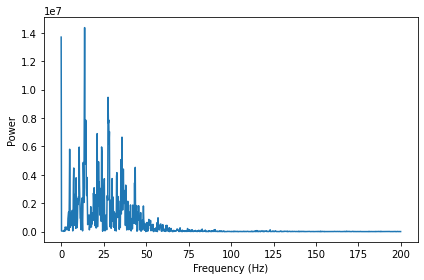
\includegraphics[scale=1]{fig/lab04/lab04_01.png}
		\caption{График сигнала}
	\end{center}
\end{figure}


\begin{lstlisting}[language=Python]
spec.plot_power()
log_wind = dict(xscale='log', yscale='log')
decorate(xlabel='Frequency (Hz)', ylabel='Power', **log_wind)
\end{lstlisting}

\begin{figure}[H]
	\begin{center}
		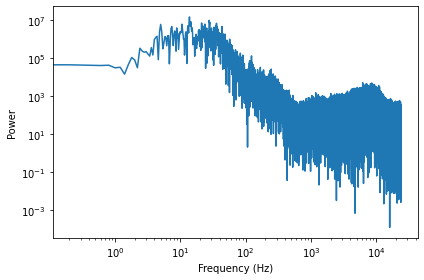
\includegraphics[scale=1]{fig/lab04/lab04_02.png}
		\caption{Спектр в логорифмическом масштабе}
	\end{center}
\end{figure}

Похоже на Броуновский шум


\begin{lstlisting}[language=Python]
spec = wave_rain.make_spectrum()
spec.plot_power(high = 200)
decorate(xlabel='Frequency (Hz)', ylabel='Power')

\end{lstlisting}

\begin{figure}[H]
	\begin{center}
		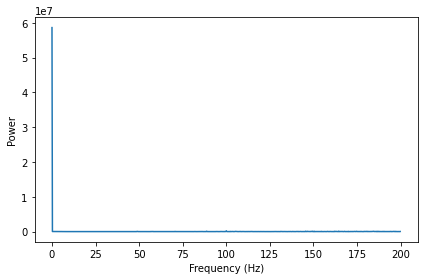
\includegraphics[scale=1]{fig/lab04/lab04_03.png}
		\caption{График сигнала}
	\end{center}
\end{figure}

\begin{lstlisting}[language=Python]
spec.plot_power()
log_rain = dict(xscale='log', yscale='log')
decorate(xlabel='Frequency (Hz)', ylabel='Power', **log_rain)
\end{lstlisting}

\begin{figure}[H]
	\begin{center}
		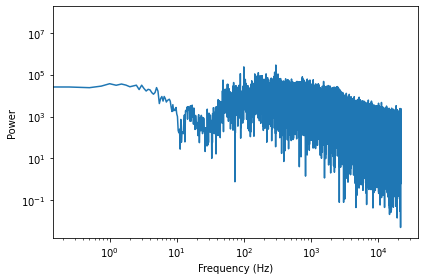
\includegraphics[scale=1]{fig/lab04/lab04_04.png}
		\caption{Спектр в логорифмическом масштабе}
	\end{center}
\end{figure}

Шум дождя тоже

\subsection{Упражнение 2}

Необходимо создать функцию, которая реализует метод Бартлетта

\begin{lstlisting}[language=Python]
def bar_method(wave, seg_length = 512, win_flag = True):
    spectogramm = wave.make_spectrogram(seg_length, win_flag)
    spec_vals = spectogramm.spec_map.values()

    psds = [spectrum.power for spectrum in spec_vals]
    hs = np.sqrt(sum(psds) / len(psds))
    fs = next(iter(spec_vals)).fs

    return thinkdsp.Spectrum(hs, fs, wave.framerate)
\end{lstlisting}

Протестируем

\begin{lstlisting}[language=Python]
psd = bar_method(wave_rain)
psd.plot_power()
log_test_1 = dict(xscale='log', yscale='log')
decorate(xlabel='Frequency (Hz)', ylabel='Power', **log_test_1)
\end{lstlisting}

\begin{figure}[H]
	\begin{center}
		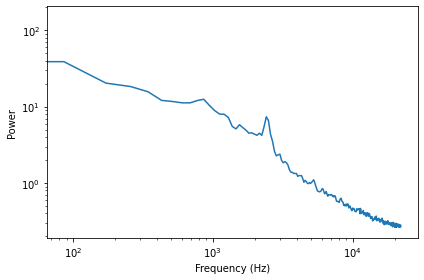
\includegraphics[scale=1]{fig/lab04/lab04_05.png}
		\caption{Результаты применения функции}
	\end{center}
\end{figure}

\begin{lstlisting}[language=Python]
psd = bar_method(wave_wind)
psd.plot_power()
log_test_2 = dict(xscale='log', yscale='log')
decorate(xlabel='Frequency (Hz)', ylabel='Power', **log_test_2)
\end{lstlisting}

\begin{figure}[H]
	\begin{center}
		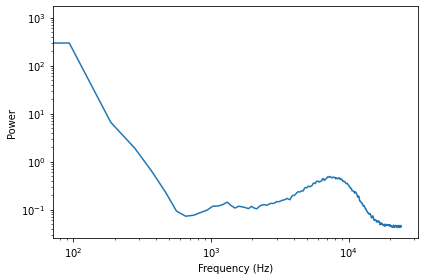
\includegraphics[scale=1]{fig/lab04/lab04_06.png}
		\caption{Результаты применения функции}
	\end{center}
\end{figure}


\subsection{Упражнение 3}

Скачаем данные по цене биткоина и вычислим его спектр

\begin{lstlisting}[language=Python]
if not os.path.exists('BTC_USD_2013-10-01_2020-03-26-CoinDesk.csv'):
    !wget https://github.com/AllenDowney/ThinkDSP/raw/master/code/BTC_USD_2013-10-01_2020-03-26-CoinDesk.csv
    
import pandas as pd

df = pd.read_csv('BTC_USD_2013-10-01_2020-03-26-CoinDesk.csv', parse_dates=[0])
df
\end{lstlisting}

\begin{figure}[H]
	\begin{center}
		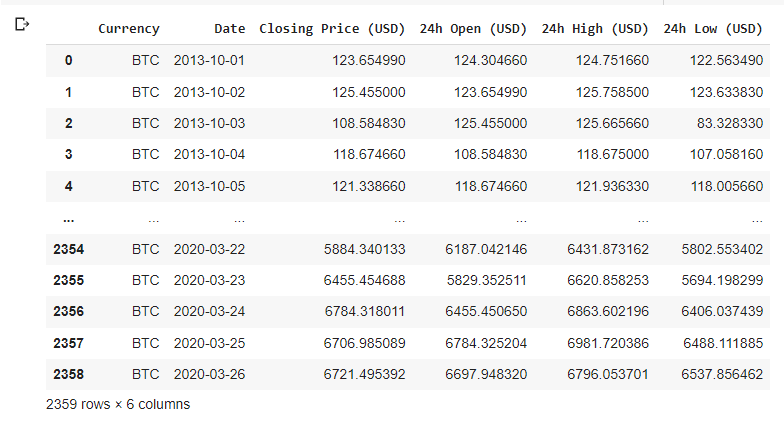
\includegraphics[scale=1]{fig/lab04/lab04_07.png}
		\caption{Таблица значений}
	\end{center}
\end{figure}

\begin{lstlisting}[language=Python]
ys = df['Closing Price (USD)']
ts = df.index

wave = thinkdsp.Wave(ys, ts, framerate = 1)
wave.plot()
decorate(xlabel='Дни')
\end{lstlisting}

\begin{figure}[H]
	\begin{center}
		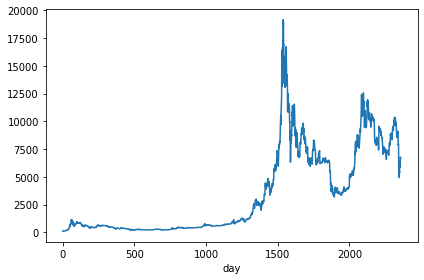
\includegraphics[scale=1]{fig/lab04/lab04_08.png}
		\caption{График цен BitCoin}
	\end{center}
\end{figure}

\begin{lstlisting}[language=Python]
spec = wave.make_spectrum()
spec.plot_power()
loglog = dict(xscale='log', yscale='log')
decorate(xlabel='Frequency (1/days)',
         ylabel='Power', 
         **loglog)
\end{lstlisting}

\begin{figure}[H]
	\begin{center}
		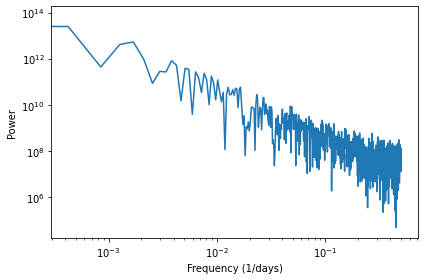
\includegraphics[scale=1]{fig/lab04/lab04_09.png}
		\caption{Спектрограмма цен BitCoin в логорифмическом формате}
	\end{center}
\end{figure}

\begin{lstlisting}[language=Python]
spec.estimate_slope()[0]

-1.7986681316517856
\end{lstlisting}

Похоже на розовый шум, так как наклон красного -2


\subsection{Упражнение 4}

Счетчик Гейгера — это прибор, который регистрирует радиацию. Когда ионизирующая частица попадает на детектор, он генерирует всплеск тока. Общий вывод в определенный момент времени можно смоделировать как некоррелированный шум Пуассона (UP), где каждая выборка представляет собой случайную величину из распределения Пуассона, которая соответствует количеству частиц, обнаруженных в течение интервала.

Напишем класс UncorrelatedPoissonNoise с наследованием от _Noise

\begin{lstlisting}[language=Python]
from thinkdsp import Noise

class UncorrelatedPoissonNoise(Noise):
    def evaluate(self, ts):
      ys = np.random.poisson(self.amp, len(ts))
      return ys
\end{lstlisting}

Проверим работу класса на значениях малой и большой амплитуды

\begin{lstlisting}[language=Python]
signal = UncorrelatedPoissonNoise(amp = 0.001)
wave = signal.make_wave(duration = 2, framerate = 10000)
wave.make_audio()

spec = wave.make_spectrum()
spec.plot_power()
decorate(xlabel='Frequency (Hz)', ylabel='Power', **loglog)
\end{lstlisting}

\begin{figure}[H]
	\begin{center}
		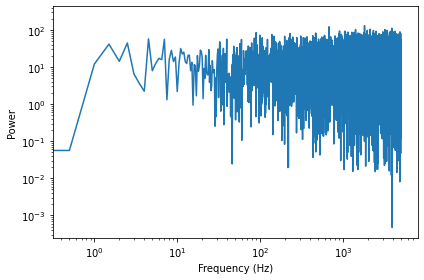
\includegraphics[scale=1]{fig/lab04/lab04_10.png}
		\caption{Получившийся спектр сигнала}
	\end{center}
\end{figure}

Теперь создадим такой же сигнал, но с большей амплитудой

\begin{lstlisting}[language=Python]
signal = UncorrelatedPoissonNoise(amp = 0.1)
wave = signal.make_wave(duration = 2, framerate = 10000)
wave.make_audio()

spec = wave.make_spectrum()
spec.plot_power()
decorate(xlabel='Frequency (Hz)', ylabel='Power', **loglog)
\end{lstlisting}

\begin{figure}[H]
	\begin{center}
		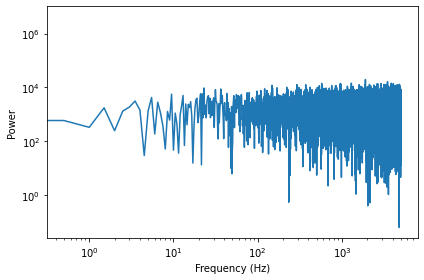
\includegraphics[scale=1]{fig/lab04/lab04_11.png}
		\caption{Получившийся спектр сигнала}
	\end{center}
\end{figure}

При малой амплитуде слышим треск как счетчик Гейгера, при большой, он становится похож на белый шум


\subsection{Упражнение 5}

В этой главе описан алгоритм генерации розового шума. Концептуально простой, но вычислительно затратный. Есть более эффективные альтернативы, такие как алгоритм Восса-Маккартни.

\noindent Исследуйте этот метод, реализуйте его, вычислите спектр и подтвердите, что он имеет желаемое отношение между мощностью и частотой.

Создадим функцию voss.

\begin{lstlisting}[language=Python]
def voss(nrows, ncols=16):

    array = np.empty((nrows, ncols))
    array.fill(np.nan)
    array[0, :] = np.random.random(ncols)
    array[:, 0] = np.random.random(nrows)
    
    n = nrows
    cols = np.random.geometric(0.5, n)
    cols[cols >= ncols] = 0
    rows = np.random.randint(nrows, size=n)
    array[rows, cols] = np.random.random(n)

    df = pd.DataFrame(array)
    df.fillna(method='ffill', axis=0, inplace=True)
    total = df.sum(axis=1)

    return total.values
\end{lstlisting}

Протестируем

\begin{lstlisting}[language=Python]
ys = voss(10000)
ys

array([8.05587101, 6.94436007, 6.57274844, ..., 7.95820399, 8.83511144,
       8.77457504])
       
wave = thinkdsp.Wave(ys)
wave.unbias()
wave.normalize()
wave.plot()
\end{lstlisting}

\begin{figure}[H]
	\begin{center}
		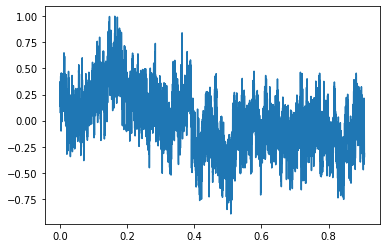
\includegraphics[scale=1]{fig/lab04/lab04_12.png}
		\caption{Сгенерированный сигнал}
	\end{center}
\end{figure}

Получаем какой-то случайный шум

\begin{lstlisting}[language=Python]
spec = wave.make_spectrum()
spec.hs[0] = 0
spec.plot_power()
decorate(xlabel='Frequency (Hz)',ylabel='Power',**loglog)
\end{lstlisting}

\begin{figure}[H]
	\begin{center}
		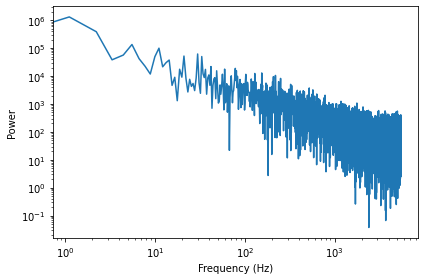
\includegraphics[scale=1]{fig/lab04/lab04_13.png}
		\caption{Спектр полученного шума}
	\end{center}
\end{figure}

\begin{lstlisting}[language=Python]
spec.estimate_slope().slope

-1.0346367430959535
\end{lstlisting}

Расчетный наклон близок к -1. Проверим на методе Бартлетта

\begin{lstlisting}[language=Python]
spec_2 = bar_method(wave, seg_length=8000, win_flag=False)
spec_2.hs[0] = 0
spec_2.plot_power()
decorate(xlabel='Frequency (Hz)', ylabel='Power', **loglog)
\end{lstlisting}


\begin{figure}[H]
	\begin{center}
		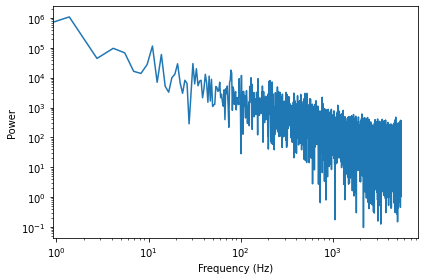
\includegraphics[scale=1]{fig/lab04/lab04_14.png}
		\caption{Спектр средней мощности шума}
	\end{center}
\end{figure}

\begin{lstlisting}[language=Python]
spec_2.estimate_slope().slope

-1.0262915371386319
\end{lstlisting}

Получаем значение чуть ближе к -1


\subsection{Вывод}

В этой работе был рассмотрен шум. Шум - сигнал, содержащий компоненты с самыми разными частотами, но не имеющий гармонической структуры периодических сигналов, рассмотреных в предыдущих работах.